\chapter{\label{chap:related-work}Trabalhos Relacionados}
As tarefas de criar uma inteligência artificial para personagens em jogos
digitais e de criar agentes inteligentes capazes de aprender a jogar jogos
digitais já foram exploradas em outros trabalhos. Neste capítulo, selecionamos
três trabalhos que se propuseram a resolver estas tarefas, indicando sua
relevância e similaridade com o projeto presente neste trabalho. 


%----------
\section{Handling Complexity in the Halo 2 AI}
A criação de agentes inteligentes com comportamentos cada vez mais complexos é
uma busca constante para desenvolvedores de jogos digitais. Criar comportamentos
complexos, contudo, vem com um preço -- que muitas vezes o desenvolvedor não
pode pagar --, como a falta de escalabilidade da arquitetura, mais tempo de
processamento ou até mesmo uma experiência ruim de interação entre jogador e
agentes inteligentes.

Este artigo é uma tentativa de elaborar um formalismo de inteligência
artificial, as \textit{Behavior Trees}, para auxiliar na criação de
comportamentos inteligentes para agentes em jogos digitais que sejam de
processamento rápido e ao mesmo tempo sofisticados, fáceis de controlar e
modularizados. As \textit{Behavior Trees} foram utilizadas para desenvolver os
comportamentos dos agentes no jogo \textit{Halo 2}, da desenvolvedora
\textit{Bungie}, e apresentaram resultados muito satisfatórios\cite{Halo2AI}.

Uma \textit{Behavior Tree} é uma estrutura de dados baseado em árvore que
consiste na organização, seleção e execução de \textbf{comportamentos} que o
agente pode executar. Cada comportamento possui uma pré-condição para executar e
uma ação, especificando como o agente atuará para este comportamento. A cada
etapa de execução, o algoritmo examina as pré-condições dos comportamentos e
decide qual comportamento é o mais adequado para executar. Esta técnica está em
rápida ascenção, pois se comparado a máquinas de estados finitos, uma técnica
muito utilizada pela indústria de jogos, são mais modulares e
extensíveis\cite{Rabin:2015:GAP:2821138}.

Esta técnica não é utilizada para criação de agentes inteligentes que jogam
jogos digitais, e sim para criação de comportamentos de agentes. Contudo, não
deixa de ser interessante para este trabalho porque, se comparado a técnicas de
inteligência artificial que envolvem treinamento, permite um controle maior
sobre os comportamentos que a inteligência artificial executa. É possível que,
se adaptada corretamente, o uso desta técnica resulte no sucesso de criação de
\textit{bots}, pois a inteligência artificial, em sua síntese, estaria
executando um comportamento no final das contas.


%----------
\section{Playing Atari with Deep Reinforcement Learning}
O artigo apresenta um modelo de \textit{deep learning} capaz de aprender
políticas de controle para sete jogos do \textit{console} Atari 2600, criando
uma inteligência artificial capaz de jogar eficientemente todos os jogos,
inclusive superando jogadores humanos em alguns
deles\cite{DBLP:journals/corr/MnihKSGAWR13}. O modelo utiliza aprendizado por
reforço e uma rede neural convolucional treinada com uma variante de
\textit{Q-learning} para criar o agente.

Para criar estas políticas de controle, os autores utilizaram uma plataforma de
testes de inteligência artificial chamada \textit{Arcade Learning
Environment}\footnote{http://www.arcadelearningenvironment.org/}.  A cada passo
de execução, o agente interage com o emulador, recebendo informações do estado
do jogo e enviando os comandos que deseja executar. As informações recebidas
eram um vetor dos \textit{pixels} apresentados na tela, o conjunto de de ações
possíveis para o jogo em questão e um valor de recompensa quando a pontuação do
jogo era alterada.

Como as informações do estado do jogo eram altamente dimensionais -- 33600
\textit{pixels} de informação visual --, foi necessário realizar um
pré-processamento para reduzir a dimensionalidade do estado do jogo -- reduzindo
para 7600 \textit{pixels}. Mesmo com esta redução, a quantidade de informações
recebidas ainda era consideravelmente grande. Por isto, a utilização de
\textit{deep learning} e redes neurais convolucionais provou ser uma excelente
-- e necessária -- escolha para realizar o treinamento do agente. Contudo, o
treinamento do agente utilizando esta técnica é extremamente demorado.

Como a dimensionalidade do estado do jogo fornecido pela ferramenta
\textit{SpelunkBots} não é tão grande quanto a do trabalho em questão, optamos
por não fazer uso de \textit{deep learning}, mesmo que a técnica também seja
muito promissora.


%----------
\section{A Neuroevolution Approach to General Atari Game Playing}
Este artigo \cite{NeuroEvolutionAtari} apresenta uma série de abordagens
neuroevolutivas para realizar a criação de agentes inteligentes capazes de
aprender a jogar jogos do \textit{console} \textit{Atari 2600} com pouco
conhecimento específico sobre os domínios dos jogos. Para criar estas políticas
de controle, os autores utilizaram uma plataforma de testes de inteligência
artificial chamada \textit{Arcade Learning Environment}.

Os autores realizaram testes com quatro algoritmos neuroevolutivos, que
descrevem redes neurais artificiais e a evolução de seus componentes:
\textit{Conventional Neuroevolution}, (CNE) \textit{Covariance Matrix Adaptation
Evolution Strategy} (CMA-ES), \textit{Neuroevolution of Augmenting Topologies}
(NEAT) e \textit{Hypercube-based Neuroevolution of Augmenting Topologies}
(HyperNEAT). Os dois primeiros algoritmos evoluem somente os pesos da rede,
enquanto que os dois últimos evoluem os pesos e a topologia da rede. O único
algoritmo que utiliza uma representação genética indireta é o \textit{HyperNEAT}
(os outros representam diretamente).

A representação de estados dos jogos foi feita de três maneiras distintas:
objetos da tela de jogo, os \textit{pixels} da tela e ruído. A representação de
objetos é a representação de mais alto nível, pois apresenta uma caracterização
informativa e clara da informação visual do jogo. A representação por
\textit{pixels} é uma representação de baixo nível, pois provê as informações
cruas da tela para o agente. É o tipo de representação mais genérico e o mais
fácil de ser aplicado para diversos jogos, e imita as informações que um jogador
humano utilizaria se estivesse jogando.  Foi necessário realizar um
\textit{downsampling}\footnote{Processo de reduzir a taxa de amostragem de um
sinal. Geralmente é aplicado para reduzir a taxa e o tamanho dos dados
recebidos.} dos valores de \textit{pixels} da tela, pois o espaço de estados era
muito grande. A representação por ruído foi utilizada para servir como base de
comparação e investigar quanto do aprendizado é baseado na memorização e em
conceitos gerais.

Foi identificado, após análise dos dados coletados, que que os algoritmos
neuroevolutivos que utilizam condificação genética direta tendem a obter
melhores resultados quando uma representação compacta de estados (objetos da
tela de jogo) é utilizada, enquanto que os algoritmos neuroevolutivos que
utilizam codificação genética indireta permitem a utilização de uma
representação com maior número de dimensões (como os \textit{pixels} da tela).
Os algoritmos com os melhores resultados, em todas as categorias de
representação de estados, foram o \textit{NEAT} e o \textit{HyperNEAT}.

Os autores descrevem que o uso de neuroevolução ajuda a diminiur os problemas
que as abordagens anteriores de criação de agentes jogadores baseadas em
\textit{Temporal Difference Learning} sofriam, como um grande espaço de estados
e gradientes de recompensa esparsas (ambos encontrados em jogos de
\textit{Atari}). Além disso, as políticas de controle evoluídas através de
algoritmos neuroevolutivos atingem resultados excelentes e, em alguns jogos,
superam o desempenho de jogadores humanos, sugerindo que a neuroevolução é uma
abordagem promissora para criação de agentes inteligentes e \textit{general
video game playing} (criar um agente que seja capaz de jogar diversos jogos
digitais sem mudanças de parâmetros).


%----------
\section{MarI/O}
Em junho de 2015, o canal do \textit{YouTube}
SethBling\footnote{https://www.youtube.com/user/sethbling/about} -- conhecido
por publicar vídeos de modificações de jogos como Mario e Minecraft -- divulgou
o vídeo \textit{MarI/O - Machine Learning for Video
Games}\footnote{https://www.youtube.com/watch?v=qv6UVOQ0F44}, que mostra um
jogador muito habilidoso completando o nível \textit{Donut Plains 1} de
\textit{Super Mario World}. É explicado, então, que o jogador em questão não é
humano, mas sim um programa de computador. Utilizando um emulador de
\textit{consoles} chamado
\textit{BizHawk}\footnote{http://tasvideos.org/BizHawk.html}, a linguagem de
programação \textit{Lua} e uma técnica de inteligência artificial chamada
\textit{\textbf{NEAT}} (\textit{NeuroEvolution of Augmenting Topologies})
\cite{stanley:ec02} -- explicada detalhadamente no capítulo \ref{chap:theory}
--, o autor programou um \textit{bot} capaz de aprender como jogar o nível em
questão do início ao fim com sucesso. Como é explicado no vídeo, inicialmente o
\textit{bot} não conhecia absolutamente nada sobre como jogar \textit{Super
Mario World}. Contudo, através de várias simulações, adquiriu o conhecimento
necessário para superar todos os obstáculos presentes no nível.

\begin{figure}[htb!]
\centering
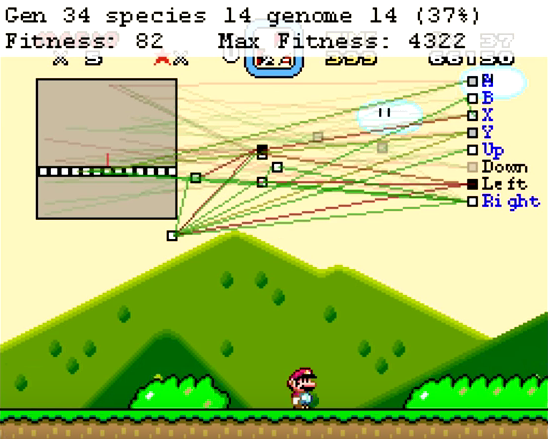
\includegraphics[width=.65\textwidth]{fig/mar-io-example.png}
\caption{\label{fig:mar-io-example}Exemplo da visão do jogo \textit{Super
Mario World} através do projeto \textit{MarI/O}, mostrando elementos de
controle usados pelo NEAT, como a rede neural, as possíveis ações, as
gerações, as espécies, os genomas, entre outros.}
\end{figure}

Depois do sucesso no nível \textit{Donut Plains 1}, o autor realizou mais
experimentos da aplicação da técnica
\textit{NEAT}\footnote{https://www.youtube.com/watch?v=iakFfOmanJU}
\footnote{https://www.youtube.com/watch?v=S9Y\_I9vY8Qw}. Inicialmente, testou em
dois outros níveis de \textit{Super Mario World}. Em \textit{Donut Plains 4}, o
processo de aprendizagem foi complicado, pois para obter progresso no nível era
necessário que aprendesse a interagir com certos elementos do mapa, e o autor
decidiu abortar o processo de aprendizagem. Já em \textit{Yoshi's Island 1},
obteve sucesso e foi capaz de concluir o nível. Com os testes finalizados, o
autor decidiu aplicar a técnica em outros dois jogos da franquia \textit{Mario}.
Em \textit{Super Mario Bros}, o \textit{bot} concluiu o primeiro nível e,
surpreendentemente, foi capaz de descobrir um \textit{glitch} no jogo que o
permitia passar por um segmento do segundo nível com maior rapidez. Em
\textit{Super Mario Kart}, depois de receber treinamento, o \textit{bot} foi
capaz de terminar uma corrida no nível \textit{Mario Circuit 1} em primeiro
lugar contra outros jogadores controlados pelo computador -- na dificuldade mais
fácil do jogo.

O \textit{MarI/O} é especialmente interessante e relevante porque tem um
objetivo muito similar ao deste trabalho: criar uma inteligência artificial
capaz de jogar uma partida de um jogo. Contudo, nos jogos escolhidos por
SethBling, os níveis são sempre os mesmos, o que torna mais fácil medir o
desempenho de um \textit{bot}, pois a disposição do nível é sempre igual e o
objetivo final sempre se encontra no mesmo lugar. Este não é o caso em
\textit{Spelunky}, onde os níveis são gerados proceduralmente. Além disso, os
níveis de \textit{Super Mario World} e \textit{Super Mario Bros.} são
essencialmente horizontais, e movimentar o personagem para a direita quase
sempre garante alguma forma de progresso. Isto facilita ainda mais o processo de
treinamento dos \textit{bots}. Em \textit{Spelunky} não é possível saber de
antemão onde se encontra a saída do nível e o movimento horizontal não garante o
progresso, visto que os níveis não são essencialmente horizontais. Estes fatores
influenciam na dificuldade de realizar o treinamento dos \textit{bots}.
